% =====================================================================
%  UPI Fraud Shield ML -- master manuscript (IEEEtran, conference mode)
%  Compile: pdfLaTeX (Overleaf default).  No external image files needed:
%  every figure is native TikZ / pgfplots.  Optional harness figures
%  (results/*.png) are inserted only if the files exist.
%
\documentclass[conference]{IEEEtran}
\IEEEoverridecommandlockouts

\usepackage[T1]{fontenc}
\usepackage[utf8]{inputenc}
\usepackage{cite}
\usepackage{amsmath,amssymb}
\usepackage{graphicx}
\usepackage{booktabs,array,tabularx,multirow}
\usepackage[table]{xcolor}
\usepackage{tikz}
\usetikzlibrary{arrows.meta,positioning,calc,fit,backgrounds}
\usepackage{pgfplots}
\pgfplotsset{compat=1.18}
\usepackage{enumitem}
\usepackage{float}
\usepackage{tcolorbox}
\usepackage{microtype}
\usepackage{balance}
\usepackage{url}
\usepackage[colorlinks=true,linkcolor=navy,citecolor=navy,urlcolor=navy]{hyperref}

% ---------- palette ----------
\definecolor{navy}{RGB}{16,42,94}
\definecolor{teal}{RGB}{0,121,125}
\definecolor{amber}{RGB}{214,125,0}
\definecolor{crimson}{RGB}{176,32,48}
\definecolor{leaf}{RGB}{46,139,87}

% ---------- macros ----------
\newcommand{\rupee}{Rs.\,}
\newcolumntype{Y}{>{\raggedright\arraybackslash}X}
\newcolumntype{C}{>{\centering\arraybackslash}X}
\setlist{nosep,leftmargin=*,itemsep=1pt}
\renewcommand{\arraystretch}{1.12}
\newcommand{\tabfont}{\footnotesize}
\hypersetup{pdftitle={UPI Fraud Shield ML},pdfauthor={Authors}}

% optional harness figure: prints nothing if the file is absent
\newcommand{\optfig}[4]{\IfFileExists{#1}{%
  \begin{figure}[!t]\centering\includegraphics[width=\columnwidth]{#1}%
  \caption{#2}\label{#3}\end{figure}}{}}

\pgfplotsset{every axis/.append style={
  tick label style={font=\scriptsize}, label style={font=\scriptsize},
  legend style={font=\scriptsize}, title style={font=\scriptsize\bfseries},
  grid=major, grid style={gray!25}}}

\tikzset{
  box/.style={draw=navy,rounded corners=2pt,fill=navy!7,align=center,font=\scriptsize,minimum height=0.8cm,inner sep=3pt},
  hot/.style={box,draw=amber,fill=amber!14},
  cool/.style={box,draw=teal,fill=teal!10},
  arr/.style={-{Stealth[length=4pt]},draw=navy!80,thick},
}

\begin{document}

\title{UPI Fraud Shield ML: A Leakage-Resistant, Explainable Machine Learning Framework for Real-Time UPI Payment Fraud Detection and Pre-Authorization Risk Stratification}

\author{\IEEEauthorblockN{Author 1, Author 2, Author 3, Author 4}
\IEEEauthorblockA{Department of Computer Science / Information Technology\\
{[Institution Name]}, India\\
Email: {[author emails]}}}

\maketitle

\begin{abstract}
UPI settles more than twelve billion payments a month on irrevocable, 24$\times$7 rails, so fraud must be stopped before authorization. This paper presents \textbf{UPI Fraud Shield ML}, a leakage-resistant, explainable framework for pre-authorization risk scoring. We (i)~define an admissibility test and a three-class leakage taxonomy and apply them to a 26,393-record synthetic corpus, retaining 36 pre-authorization predictors; (ii)~confine SMOTE to the 80\% training split so that the 5,279-record test set (909 fraud) keeps its native 17.22\% prevalence; and (iii)~benchmark five classifiers. Gradient Boosting reaches F1 99.95\% (1 false positive, 0 false negatives) and the deployed Random Forest 99.89\% (2 FP, 0 FN, ROC-AUC 1.0000); the gap is one transaction and statistically indistinguishable (exact McNemar $p=1.0$). Because a linear model already reaches AUC 0.9999, we read these scores as evidence of synthetic separability, not deployable accuracy: at fixed error rates, Random Forest precision falls from 99.78\% to 68.6\% at 0.1\% fraud prevalence. Predictions map to four risk bands with SHAP explanations and rule-based precautions. We close with a threat model, a validity audit, calibration and out-of-time validation protocols, and an enterprise streaming roadmap.
\end{abstract}

\begin{IEEEkeywords}
UPI fraud detection, pre-authorization risk scoring, target leakage, SMOTE, explainable AI, SHAP, probability calibration, cost-sensitive learning
\end{IEEEkeywords}

% =====================================================================
\section{Introduction}
\subsection{The UPI setting}
UPI is layered on the IMPS interbank switch operated by the National Payments Corporation of India (NPCI)~\cite{npci}. A payer's app resolves a virtual payment address (VPA, \texttt{name@\allowbreak{}handle}) to an account, the issuing bank verifies a UPI PIN, and the debit and credit legs settle in near real time, around the clock. Three properties shape the fraud problem. Settlement is effectively \emph{irrevocable}: recovery depends on receiver cooperation and dispute workflows rather than a scheme-mediated chargeback. VPAs \emph{decouple identity from account number}, making receiver identities cheap to create and rotate. And \emph{pull flows exist}: a collect request lets an attacker disguise a debit as an incoming credit.

Card regimes can lean on retrospective chargebacks. On instant rails that second layer largely disappears, so the one high-value control point is the interval between payload receipt and authorization. A pre-authorization scorer must therefore use only information available before authorization, respond within the payment's latency budget, and emit a \emph{graded} action (approve, step-up, hold, block), because a wrongful block is felt immediately by a legitimate user.

\subsection{Threat vectors}
Five vectors organize the feature design and test cases of this paper:
\begin{enumerate}
\item \textbf{SIM-swap / device relay.} A duplicate SIM lets an attacker bind the victim's VPA to a new handset and receive OTPs, producing OTP--device inconsistency and geographic/IP disparity.
\item \textbf{Collect-request spoofing.} A request to pay is presented as a refund; the victim approves and enters a PIN, authorizing a debit.
\item \textbf{Fake merchant QR.} An attacker's QR overlays a merchant's, so the receiving handle's name, category and history do not match the claimed business.
\item \textbf{Vishing / social engineering.} The victim, coached by phone, operates their own device, so device and biometric signals look legitimate.
\item \textbf{Digital-arrest scams and mule rings.} Victims coerced by impersonated authorities push funds to accounts that fan money out through short cyclic paths.
\end{enumerate}

\subsection{Why rules alone are not enough}
Static rules (amount ceilings, velocity limits, blacklists) are transparent and cheap but encode their authors' assumptions and decay silently as attackers adapt~\cite{bolton02,chandola09}. Supervised models capture conjunctions rules miss, for example a moderate amount that becomes suspicious only alongside an OTP--device mismatch. Because the scores gate real payments, they must also be explainable to analysts and auditors~\cite{lundberg17,lundberg20}.

\subsection{Contributions}
\begin{enumerate}
\item A \textbf{leakage-resistance protocol}: a formal admissibility test, a three-class leakage taxonomy, and an audit that removed variables synthetically coupled to the label.
\item A \textbf{36-feature, six-category pre-authorization representation} with a pipeline in which SMOTE, encoding and scaling are fit on training data only, plus the prior-shift correction needed to turn balanced-training scores into operational risk bands.
\item A \textbf{rigorous benchmark} of five model families on a pristine test set: exact confusion decomposition, cost-dominance analysis, prevalence-shifted precision and exact paired tests.
\item An \textbf{explainability and precaution layer} pairing SHAP with percentile-specified alerts, traced end-to-end on three threat scenarios.
\item A frank \textbf{validity audit and enterprise roadmap} that states the limits of near-perfect synthetic scores.
\end{enumerate}

\begin{tcolorbox}[colback=navy!5,colframe=navy,boxrule=0.6pt,arc=2pt,left=4pt,right=4pt,top=2pt,bottom=2pt,title={\footnotesize\bfseries Key results at a glance},fonttitle=\footnotesize,coltitle=white]
\footnotesize
\begin{itemize}[leftmargin=1.2em]
\item Best F1: \textbf{Gradient Boosting 99.95\%} (1 FP, 0 FN); deployed \textbf{Random Forest 99.89\%} (2 FP, 0 FN).
\item RF vs.\ GB differ by \textbf{one test record}; exact McNemar $p=1.0$.
\item Logistic Regression alone: \textbf{AUC 0.9999} $\Rightarrow$ near-linear synthetic separability.
\item RF precision \textbf{99.78\% $\rightarrow$ 68.6\%} when prevalence falls from 17.22\% to 0.1\%.
\end{itemize}
\end{tcolorbox}

% =====================================================================
\section{Problem Formulation and Threat Model}
Let $\mathbf{x}\in\mathbb{R}^{36}$ be the encoded pre-authorization vector and $y\in\{0,1\}$ the fraud label, with prevalence $\pi=4{,}545/26{,}393=0.1722$. A scorer returns $\hat p(\mathbf{x})\approx P(y{=}1\mid\mathbf{x})$. In plain terms, the model is mathematically penalized more heavily for missing a fraud than for slightly inconveniencing a legitimate user. Formally, if $C_{\text{FN}}$ and $C_{\text{FP}}$ are the costs of a missed fraud and a wrongful interruption, the cost-sensitive logistic objective, with $f_i=f_\theta(\mathbf{x}_i)$, is
\begin{equation}
\mathcal{L}(\theta)=\sum_{i=1}^{N}\Big[y_iC_{\text{FN}}\log\!\big(1{+}e^{-f_i}\big)+(1{-}y_i)C_{\text{FP}}\log\!\big(1{+}e^{f_i}\big)\Big],
\end{equation}
and, for a calibrated posterior, the Bayes-optimal decision threshold is
\begin{equation}
t^\star=\frac{C_{\text{FP}}}{C_{\text{FP}}+C_{\text{FN}}}=\frac{1}{1+\rho},\qquad \rho=\frac{C_{\text{FN}}}{C_{\text{FP}}}.
\end{equation}
Three consequences matter below.

\textbf{(a) Class weights are an implicit threshold.} Scikit-learn's \texttt{balanced} weights imply $\rho=21{,}848/4{,}545=4.807$, i.e.\ $t^\star=\pi=0.1722$. On the SMOTE-balanced training set ($n_0=n_1=17{,}478$) the balanced weights are exactly 1, so \texttt{class\_\allowbreak{}weight='balanced'} becomes a \emph{no-op} once models are fit on resampled data.

\textbf{(b) The risk bands encode cost asymmetries.} Read through Eq.~(2), the band edges $0.2$, $0.5$ and $0.8$ correspond to $\rho=4$, $1$ and $0.25$ (Fig.~\ref{fig:bands}): a step-up challenge is optimal when a missed fraud costs at least four times a challenge, and blocking is optimal only when a wrongful block costs at least four times a missed fraud.

\textbf{(c) Prior shift.} A model trained at prior $\pi_s$ and deployed at $\pi_d$ needs its odds rescaled:
\begin{equation}
\frac{q_d}{1-q_d}=\frac{\hat p_s}{1-\hat p_s}\cdot\frac{\pi_d/(1-\pi_d)}{\pi_s/(1-\pi_s)}.
\end{equation}
For SMOTE training ($\pi_s=0.5$) the odds are multiplied by $\pi_d/(1-\pi_d)$: 0.208 at the corpus prevalence and 0.001 at $\pi_d=0.1\%$. Uncorrected scores overstate risk and push traffic into higher bands.

\begin{figure}[!t]
\centering
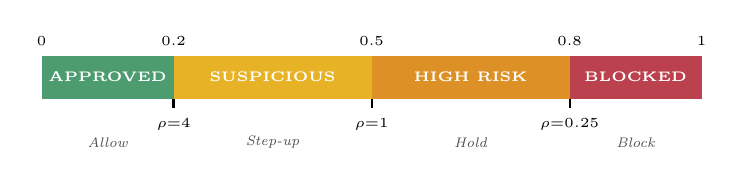
\begin{tikzpicture}[x=3.3in]
  \foreach \a/\b/\c/\t in {0/0.2/leaf/APPROVED, 0.2/0.5/amber!70!yellow/SUSPICIOUS, 0.5/0.8/amber/{HIGH RISK}, 0.8/1/crimson/BLOCKED}{
    \fill[\c!85] (\a,0) rectangle (\b,0.55);
    \node[font=\tiny\bfseries,white] at ({(\a+\b)/2},0.275) {\t};}
  \foreach \p/\r in {0.2/4, 0.5/1, 0.8/0.25}{
    \draw[thick] (\p,0) -- (\p,-0.12);
    \node[font=\tiny,below] at (\p,-0.12) {$\rho{=}\r$};}
  \foreach \p in {0,0.2,0.5,0.8,1}{\node[font=\tiny,above] at (\p,0.55) {\p};}
  \foreach \p/\t in {0.1/Allow,0.35/Step-up,0.65/Hold,0.9/Block}{\node[font=\tiny\itshape,gray!60!black] at (\p,-0.55) {\t};}
\end{tikzpicture}
\caption{Four-band risk operator on the calibrated probability $\hat p$, with the cost ratio $\rho=C_{\text{FN}}/C_{\text{FP}}$ implied at each band edge by Eq.~(2).}
\label{fig:bands}
\end{figure}

\subsection{Adversary model}
Features split by \emph{who controls them}: attacker-controllable (amount, request cadence, handle attributes), victim-generated (typing speed, device, session) and system-immutable within a session (sender history, account age). Table~\ref{tab:adv} lists the four adversary classes. We assume Kerckhoffs conditions: attackers know the feature families but not the learned parameters and may probe the scorer a bounded number of times. The key design implication is that in vishing the \emph{victim} generates the device and biometric signals, so those channels become uninformative and the model must lean on counterparty and amount-deviation signals.

\begin{table}[!t]
\caption{Adversary classes}\label{tab:adv}
\centering\tabfont
\begin{tabularx}{\columnwidth}{@{}l Y Y@{}}
\toprule
\textbf{Class} & \textbf{Controls / cannot control} & \textbf{Defensive implication}\\
\midrule
A1 Scripted automation & Amount, cadence, handle string / sender history, victim device & Limit probing; hide cut-offs; rely on system-immutable features\\
A2 Social engineer & Victim's decision / victim device, receiver history & Device and biometrics uninformative; use counterparty and deviation signals\\
A3 Mule syndicate & Receiver handle, account age / sender behavior & Receiver reputation, graph features\\
A4 SIM-swap / relay & OTP channel on new handset / victim's historical device & OTP--device consistency, geographic/IP disparity\\
\bottomrule
\end{tabularx}
\end{table}

\begin{table*}[!t]
\caption{Threat-vector-to-signal mapping}\label{tab:threat}
\centering\tabfont
\begin{tabularx}{\textwidth}{@{}l Y Y c@{}}
\toprule
\textbf{Threat vector} & \textbf{What the attacker does} & \textbf{Primary detection signals} & \textbf{Groups}\\
\midrule
Phishing / collect-request spoofing & Disguises a debit as a refund or incoming credit; victim approves with a PIN & \texttt{time\_\allowbreak{}between\_\allowbreak{}link\_\allowbreak{}click\_\allowbreak{}and\_\allowbreak{}transaction}, \texttt{request\_\allowbreak{}amount\_\allowbreak{}roundness}, \texttt{requester\_\allowbreak{}account\_\allowbreak{}age}, \texttt{transaction\_\allowbreak{}amount\_\allowbreak{}vs\_\allowbreak{}sender\_\allowbreak{}history} & G4, G6, G1\\
SIM swap / device relay & Binds the victim's VPA to a new handset and intercepts OTPs & \texttt{otp\_\allowbreak{}request\_\allowbreak{}device\_\allowbreak{}consistency}, \texttt{otp\_\allowbreak{}request\_\allowbreak{}frequency}, \texttt{time\_\allowbreak{}between\_\allowbreak{}otp\_\allowbreak{}generation\_\allowbreak{}and\_\allowbreak{}input}, \texttt{geographic\_\allowbreak{}disparity}, \texttt{geographic\_\allowbreak{}location\_\allowbreak{}vs\_\allowbreak{}ip} & G2, G5\\
Fake merchant QR & Overlays a merchant's QR so payment reaches the attacker's handle & \texttt{business\_\allowbreak{}name\_\allowbreak{}match}, \texttt{handle\_\allowbreak{}similarity\_\allowbreak{}score}, \texttt{merchant\_\allowbreak{}category\_\allowbreak{}code}, \texttt{handle\_\allowbreak{}transaction\_\allowbreak{}history} & G6, G1\\
Vishing / digital arrest & Coaches the victim by phone through authorizing the transfer & \texttt{transaction\_\allowbreak{}amount\_\allowbreak{}vs\_\allowbreak{}sender\_\allowbreak{}history}, \texttt{input\_\allowbreak{}timing\_\allowbreak{}consistency}, \texttt{session\_\allowbreak{}duration}, \texttt{app\_\allowbreak{}switching\_\allowbreak{}frequency}, \texttt{relationship\_\allowbreak{}to\_\allowbreak{}requester} & G1, G3, G4\\
Mule ring & Fans stolen funds out through fresh, rotating accounts and short cycles & \texttt{upi\_\allowbreak{}handle\_\allowbreak{}age}, \texttt{handle\_\allowbreak{}transaction\_\allowbreak{}history}, \texttt{requester\_\allowbreak{}account\_\allowbreak{}age}, \texttt{transaction\_\allowbreak{}velocity} & G6, G1\\
\bottomrule
\end{tabularx}
\end{table*}

% =====================================================================
\section{Related Work}
\textbf{Fraud detection practice.} Surveys document the recurring difficulties of fraud modeling: extreme imbalance, delayed and noisy labels, cost asymmetry and adversarial drift~\cite{bolton02,phua10,ngai11,chandola09}. Practitioner studies show that label delay, concept drift and alert budgets matter more than the choice of classifier~\cite{dalpozzolo14}, that evaluation must respect the temporal structure of fraud streams~\cite{dalpozzolo18}, and that engineered aggregate and periodic behavioral features improve cost-sensitive performance~\cite{bahnsen16}.

\textbf{Models and imbalance.} Bagged and boosted trees~\cite{breiman01,friedman01,friedman02,chen16} remain strong on tabular data~\cite{grinsztajn22}. SMOTE interpolates between a minority sample and its $k$ nearest minority neighbors~\cite{chawla02}; because interpolation happens in feature space, it is sensitive to scaling and nominal encodings (Section~\ref{sec:arch}). Probability calibration interacts with rebalancing~\cite{dalpozzolo15}, and Platt scaling~\cite{platt99}, isotonic regression~\cite{zadrozny02} and cross-family comparisons~\cite{niculescu05,guo17} provide the correction toolkit; the precision--recall view is the right lens at low prevalence~\cite{davis06,saito15}.

\textbf{Leakage and explanation.} Kaufman et al.\ formalize leakage as using information in training that is unavailable, or distributed differently, at prediction time~\cite{kaufman12}. SHAP unifies additive attribution methods under the Shapley value~\cite{lundberg17,shapley53}, with exact polynomial-time computation for trees~\cite{lundberg20}; LIME is a local-surrogate alternative~\cite{ribeiro16}.

The authors are not aware of a public UPI-native dataset with behavioral telemetry, which plausibly reflects privacy and commercial constraints and motivates the synthetic-data caveats of Section~\ref{sec:threats}. Table~\ref{tab:taxonomy} positions this study.

\begin{table*}[!t]
\caption{Comparative taxonomy of representative studies}\label{tab:taxonomy}
\centering\tabfont
\begin{tabularx}{\textwidth}{@{}l Y Y Y Y Y Y@{}}
\toprule
\textbf{Study} & \textbf{Data scale} & \textbf{Feature domain} & \textbf{Model family} & \textbf{Explainability} & \textbf{Real-time SLA} & \textbf{Critical vulnerability}\\
\midrule
Bolton \& Hand~\cite{bolton02} & Survey, no single dataset & Card, telecom, insider & Statistical, outlier, supervised & Not addressed & Not addressed & Pre-dates ensembles and XAI; no leakage protocol\\
Dal Pozzolo et al.~\cite{dalpozzolo14} & Real card transactions (industrial partner) & Transaction aggregates & Ensembles under practical constraints & Not addressed & Delayed-label and alert-budget limits discussed & Proprietary data; not reproducible\\
Dal Pozzolo et al.~\cite{dalpozzolo15} & Public card subset: 284,807 txns, 492 frauds & PCA components, amount, time & Undersampling with calibration & None (anonymized) & Not reported & Obfuscated features block semantic explanation; short window\\
Bahnsen et al.~\cite{bahnsen16} & Real card data (proprietary) & Aggregated and periodic behavioral & Cost-sensitive classifiers & Not addressed & Not reported & Proprietary; no public replication\\
Chen \& Guestrin~\cite{chen16} & General benchmarks & Generic tabular & Boosted trees & Gain importance & Not fraud-specific & Importance is global and non-causal\\
Weber et al.~\cite{weber19} & Illicit-transaction graph: 203,769 nodes, 234,355 edges & Graph and node features & GCN & Limited & Not reported & Cryptocurrency AML, not instant-payment rails\\
Lundberg et al.~\cite{lundberg20} & Medical and general tabular & Generic & Tree SHAP & Exact local attribution & Polynomial-time algorithm & Not validated on fraud streams\\
\rowcolor{navy!8}\textbf{This study} & 26,393 $\times$ 65 synthetic UPI corpus (36 features) & Transaction, authentication, session, request, geographic, counterparty & LR, CART, RF, GB, MLP & SHAP plus rule-based precautions & Budget specified; one prototype measurement & Synthetic near-linear separability; random split only\\
\bottomrule
\end{tabularx}
\end{table*}

% =====================================================================
\section{Data, Leakage Audit and Features}
\subsection{Corpus}
The synthetic corpus \texttt{fraud\_\allowbreak{}dataset.csv} holds 26,393 records and 65 raw columns, with 21,848 legitimate (82.78\%) and 4,545 fraudulent (17.22\%) transactions. After the audit below, 28 columns are removed and 36 predictors remain ($65-36-1=28$). An 80:20 stratified split (\texttt{random\_\allowbreak{}state=42}) yields 21,114 training and 5,279 test records (Fig.~\ref{fig:split}); SMOTE then lifts the training set to 34,956 records by adding 13,842 synthetic frauds, while the test set stays untouched.

\begin{figure}[!t]
\centering
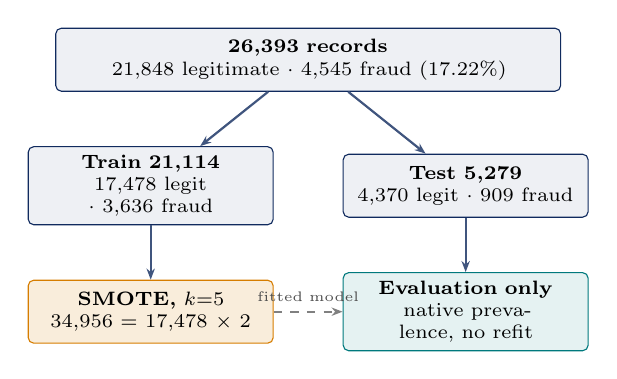
\begin{tikzpicture}[node distance=0.5cm]
  \node[box,text width=6.2cm] (all) at (0,0) {\textbf{26,393 records}\\21,848 legitimate $\cdot$ 4,545 fraud (17.22\%)};
  \node[box,text width=2.9cm] (tr) at (-2.0,-1.6) {\textbf{Train 21,114}\\17,478 legit $\cdot$ 3,636 fraud};
  \node[box,text width=2.9cm,] (te) at (2.0,-1.6) {\textbf{Test 5,279}\\4,370 legit $\cdot$ 909 fraud};
  \node[hot,text width=2.9cm,] (sm) at (-2.0,-3.2) {\textbf{SMOTE, $k{=}5$}\\34,956 = 17,478 $\times$ 2};
  \node[cool,text width=2.9cm,] (ev) at (2.0,-3.2) {\textbf{Evaluation only}\\native prevalence, no refit};
  \draw[arr] (all) -- (tr); \draw[arr] (all) -- (te);
  \draw[arr] (tr) -- (sm); \draw[arr] (te) -- (ev);
  \draw[arr,dashed,gray] (sm.east) -- node[above,font=\tiny,gray!60!black]{fitted model} (ev.west);
\end{tikzpicture}
\caption{Data partition. Oversampling touches only the training branch (13,842 synthetic frauds); the test branch is never resampled or refit.}
\label{fig:split}
\end{figure}

\subsection{Leakage audit}
A feature is \emph{admissible} only if (i)~its value is known before authorization and (ii)~its relationship to the label at deployment matches the one in training. Table~\ref{tab:leak} lists the three failure classes and what was removed.

\begin{table}[!t]
\caption{Leakage taxonomy and audit outcome}\label{tab:leak}
\centering\tabfont
\begin{tabularx}{\columnwidth}{@{}l Y Y@{}}
\toprule
\textbf{Class} & \textbf{Examples in this corpus} & \textbf{Action}\\
\midrule
I\;Post-event & Post-event variables flagged in the notebook & Removed\\
II\;Generator-coupled & \texttt{receiver\_\allowbreak{}account\_\allowbreak{}age}, \texttt{receiver\_\allowbreak{}transaction\_\allowbreak{}history} (synthetically tied to the label); \texttt{pin\_\allowbreak{}entry\_\allowbreak{}method} (correlation $\approx0.524$ with the target) & Removed\\
III\;Identifier proxy & \texttt{transaction\_\allowbreak{}id}, \texttt{user\_\allowbreak{}id}, \texttt{merchant\_\allowbreak{}id}, \texttt{timestamp}, \texttt{device\_\allowbreak{}id}, IP, location, URL referrer, free text & Removed\\
List-type fields & String-stored lists with effectively no variance & Removed\\
\bottomrule
\end{tabularx}
\end{table}

Why does leakage produce deceptive near-100\% scores? If a generator-coupled column separates the classes by five noise standard deviations, its single-feature AUC is already 0.9998 and a simple threshold errs on 0.62\% of records. A random split from the same generator cannot reveal this, because train and test share the artifact; at deployment the dependence turns into noise. The pre-audit pipeline reportedly scored approximately perfectly, and the audited pipeline \emph{still} scores near-perfectly, a persistence examined in Section~\ref{sec:threats}.

\subsection{Feature architecture}
Table~\ref{tab:feat} groups the 36 predictors into six signal categories. Group assignment follows operational semantics; 34 of the 36 predictors are named below; the remaining two are recorded in \texttt{feature\_\allowbreak{}cols.pkl}.

\begin{table*}[!t]
\caption{The 36-feature pre-authorization representation by signal group}\label{tab:feat}
\centering\tabfont
\begin{tabularx}{\textwidth}{@{}l c Y Y@{}}
\toprule
\textbf{Group} & \textbf{n} & \textbf{Features} & \textbf{Operational signal}\\
\midrule
G1 Transaction magnitude and velocity & 5 & \texttt{amount\_\allowbreak{}log}, \texttt{transaction\_\allowbreak{}amount\_\allowbreak{}vs\_\allowbreak{}sender\_\allowbreak{}history}, \texttt{transaction\_\allowbreak{}velocity}, \texttt{failed\_\allowbreak{}transaction\_\allowbreak{}count}, \texttt{transaction\_\allowbreak{}type} & Absolute and personalized deviation; burst drains; credential guessing\\
G2 Authentication and OTP & 5 & \texttt{authentication\_\allowbreak{}attempts}, \texttt{authorization\_\allowbreak{}method}, \texttt{otp\_\allowbreak{}request\_\allowbreak{}frequency}, \texttt{otp\_\allowbreak{}request\_\allowbreak{}device\_\allowbreak{}consistency}, \texttt{time\_\allowbreak{}between\_\allowbreak{}otp\_\allowbreak{}generation\_\allowbreak{}and\_\allowbreak{}input} & OTP harvesting, SIM-swap and remote relay, coached retries\\
G3 Session and behavioral biometrics & 7 & \texttt{session\_\allowbreak{}duration}, \texttt{screen\_\allowbreak{}active\_\allowbreak{}time}, \texttt{keyboard\_\allowbreak{}input\_\allowbreak{}speed}, \texttt{app\_\allowbreak{}switching\_\allowbreak{}frequency}, \texttt{input\_\allowbreak{}timing\_\allowbreak{}consistency}, \texttt{pin\_\allowbreak{}entry\_\allowbreak{}speed}, \texttt{background\_\allowbreak{}data\_\allowbreak{}usage} & Operator change, hesitation, remote-access tooling\\
G4 Request / collect behavior & 7 & \texttt{request\_\allowbreak{}frequency}, \texttt{request\_\allowbreak{}acceptance\_\allowbreak{}rate}, \texttt{time\_\allowbreak{}to\_\allowbreak{}respond\_\allowbreak{}to\_\allowbreak{}request}, \texttt{request\_\allowbreak{}amount\_\allowbreak{}roundness}, \texttt{time\_\allowbreak{}between\_\allowbreak{}link\_\allowbreak{}click\_\allowbreak{}and\_\allowbreak{}transaction}, \texttt{relationship\_\allowbreak{}to\_\allowbreak{}requester}, \texttt{dns\_\allowbreak{}lookup\_\allowbreak{}age} & Collect spam, scripted amounts, rushed approval, phishing-link flows\\
G5 Geographic context & 2 & \texttt{geographic\_\allowbreak{}disparity}, \texttt{geographic\_\allowbreak{}location\_\allowbreak{}vs\_\allowbreak{}ip} & Account takeover, proxy or relay\\
G6 Counterparty, handle and merchant & 8 & \texttt{requester\_\allowbreak{}account\_\allowbreak{}age}, \texttt{upi\_\allowbreak{}handle\_\allowbreak{}age}, \texttt{handle\_\allowbreak{}similarity\_\allowbreak{}score}, \texttt{handle\_\allowbreak{}contains\_\allowbreak{}official\_\allowbreak{}terms}, \texttt{handle\_\allowbreak{}transaction\_\allowbreak{}history}, \texttt{business\_\allowbreak{}name\_\allowbreak{}match}, \texttt{social\_\allowbreak{}media\_\allowbreak{}presence}, \texttt{merchant\_\allowbreak{}category\_\allowbreak{}code} & Fresh mule accounts, look-alike handles, fake-QR substitution\\
\bottomrule
\end{tabularx}
\end{table*}

\begin{figure}[!t]
\centering
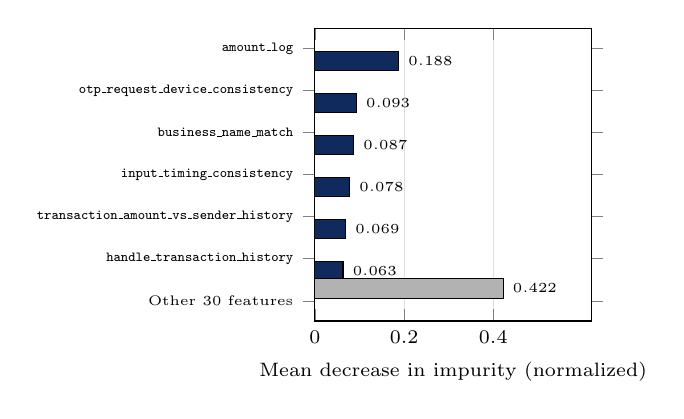
\begin{tikzpicture}
\begin{axis}[xbar,width=0.42\columnwidth,height=5.3cm,bar width=7pt,xmin=0,xmax=0.62,xtick={0,0.2,0.4},
  y dir=reverse,ytick={1,...,7},
  yticklabels={\texttt{amount\_log},\texttt{otp\_request\_device\_consistency},\texttt{business\_name\_match},\texttt{input\_timing\_consistency},\texttt{transaction\_amount\_vs\_sender\_history},\texttt{handle\_transaction\_history},Other 30 features},
  yticklabel style={font=\tiny},xlabel={Mean decrease in impurity (normalized)},
  nodes near coords,every node near coord/.append style={font=\tiny,/pgf/number format/fixed,/pgf/number format/precision=3},
  grid=none,xmajorgrids=true,enlarge y limits=0.08]
\addplot[fill=navy] coordinates {(0.188,1)(0.093,2)(0.087,3)(0.078,4)(0.069,5)(0.063,6)};
\addplot[fill=gray!60] coordinates {(0.422,7)};
\end{axis}
\end{tikzpicture}
\caption{Random Forest feature importance: six leading features hold 57.8\% of total importance; the remaining 30 share 42.2\%. Impurity importance favors continuous predictors and is not causal~\cite{strobl07}.}
\label{fig:imp}
\end{figure}

% =====================================================================
\section{Architecture and Preprocessing}\label{sec:arch}
\begin{figure*}[!t]
\centering
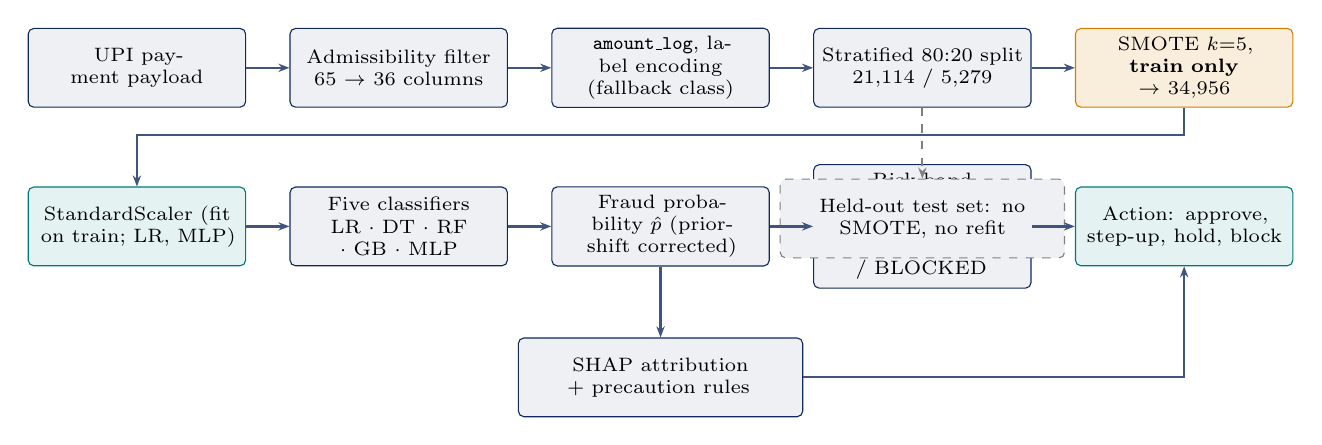
\begin{tikzpicture}[node distance=0.55cm,box/.append style={text width=2.55cm,minimum height=1.0cm}]
  \node[box] (n1) {UPI payment payload};
  \node[box,right=of n1] (n2) {Admissibility filter\\65 $\rightarrow$ 36 columns};
  \node[box,right=of n2] (n3) {\texttt{amount\_\allowbreak{}log}, label encoding (fallback class)};
  \node[box,right=of n3] (n4) {Stratified 80:20 split\\21,114 / 5,279};
  \node[hot,right=of n4] (n5) {SMOTE $k{=}5$, \textbf{train only}\\$\rightarrow$ 34,956};
  \node[cool,below=1.0cm of n1] (n6) {StandardScaler (fit on train; LR, MLP)};
  \node[box,right=of n6] (n7) {Five classifiers\\LR $\cdot$ DT $\cdot$ RF $\cdot$ GB $\cdot$ MLP};
  \node[box,right=of n7] (n8) {Fraud probability $\hat p$ (prior-shift corrected)};
  \node[box,right=of n8] (n9) {Risk band\\APPROVED / SUSPICIOUS / HIGH RISK / BLOCKED};
  \node[cool,right=of n9] (n10) {Action: approve, step-up, hold, block};
  \node[box,below=0.9cm of n8,text width=3.4cm] (n11) {SHAP attribution + precaution rules};
  \node[box,dashed,below=0.9cm of n4,text width=3.4cm,draw=gray] (te) {Held-out test set: no SMOTE, no refit};
  \foreach \a/\b in {n1/n2,n2/n3,n3/n4,n4/n5,n6/n7,n7/n8,n8/n9,n9/n10}{\draw[arr] (\a) -- (\b);}
  \draw[arr] (n5.south) -- ++(0,-0.35) -| (n6.north);
  \draw[arr] (n8) -- (n11);
  \draw[arr] (n11.east) -| (n10.south);
  \draw[arr,dashed,gray] (n4) -- (te);
\end{tikzpicture}
\caption{End-to-end pipeline. Training-only stages are highlighted; at inference the same encoders, feature order and scaler are loaded from serialized artifacts and SMOTE is never applied.}
\label{fig:pipe}
\end{figure*}

\textbf{Amount transform.} Amounts are heavy-tailed, so the pipeline uses
\begin{equation}
z=\ln\!\big(1+\max(0,x)\big).
\end{equation}
Tree models are invariant to this monotone transform; it matters for the linear and neural models and for the geometry of SMOTE interpolation.

\textbf{SMOTE.} A synthetic minority point is generated as
\begin{equation}
\mathbf{x}_{\text{new}}=\mathbf{x}_i+\lambda(\mathbf{x}_{nn}-\mathbf{x}_i),\qquad\lambda\sim\mathcal{U}(0,1),
\end{equation}
with $\mathbf{x}_{nn}$ drawn from the $k=5$ nearest minority neighbors. If oversampling preceded the split, such points would be interpolated from records that later land in the test set, giving the training data near-duplicates of test frauds and rewarding memorization; fitting SMOTE after the split closes this path.

\textbf{Three inherited caveats.}
\begin{enumerate}
\item \emph{Inert class weights.} After SMOTE the balanced class weights equal 1 (Section~II), so rebalancing is performed by SMOTE alone.
\item \emph{Neighbor search on unscaled, label-encoded data.} The scaler is fit \emph{after} SMOTE, so $k$-NN distances are dominated by large-range columns, and interpolating between integer codes of nominal columns yields fractional codes that match no category. SMOTE-NC, or scaling before SMOTE inside an \texttt{imblearn} pipeline~\cite{lemaitre17}, removes both issues.
\item \emph{MLP early-stopping leakage.} The internal 15\% validation split is drawn from the resampled set, so synthetic points sit beside their real parents on both sides, making early stopping optimistic.
\end{enumerate}

\textbf{Encoding and scaling.} Nominal predictors use \texttt{LabelEncoder}; at inference an unseen category falls back to the encoder's first known class. This avoids a crash but silently relabels novelty as a real category; production systems should reserve an explicit \texttt{UNK} level and monitor its rate as a drift signal. The \texttt{StandardScaler} is fit on the balanced training set and applied unchanged to test and inference rows; only LR and the MLP consume scaled inputs.

% =====================================================================
\section{Models}
All five classifiers use the same 36-column representation (Table~\ref{tab:models}). Logistic Regression is the transparent linear baseline~\cite{hosmer13}; CART~\cite{breiman84} gives compact non-linear rules; Random Forest~\cite{breiman01} averages bootstrapped trees to cut variance; Gradient Boosting~\cite{friedman01,friedman02} fits trees sequentially to residuals with shrinkage; and the MLP~\cite{rumelhart86} adds a learned non-linear map with L2 weight decay. Unspecified parameters take scikit-learn~\cite{pedregosa11} defaults (Appendix~A).

\begin{table*}[!t]
\caption{Model configuration}\label{tab:models}
\centering\tabfont
\begin{tabularx}{\textwidth}{@{}l Y c Y Y@{}}
\toprule
\textbf{Model} & \textbf{Hyperparameters} & \textbf{Scaled} & \textbf{Training cost} & \textbf{Inference cost}\\
\midrule
Logistic Regression & \texttt{C=0.5}, balanced, \texttt{max\_\allowbreak{}iter=1000} & Yes & $O(I\,n\,d)$, $I\le1000$ & $O(d)$\\
Decision Tree & \texttt{max\_\allowbreak{}depth=6}, \texttt{min\_\allowbreak{}samples\_\allowbreak{}leaf=20}, balanced & No & $O(d\,n\log n)$ & $O(6)$ node tests\\
Random Forest (deployed) & 200 trees, \texttt{max\_\allowbreak{}depth=8}, \texttt{min\_\allowbreak{}samples\_\allowbreak{}leaf=10}, balanced, all cores & No & $O(T\,d'\,n\log n)$, parallel in $T$ & $\approx1{,}600$ node tests\\
Gradient Boosting & 150 estimators, \texttt{learning\_\allowbreak{}rate=0.08}, \texttt{max\_\allowbreak{}depth=4}, \texttt{min\_\allowbreak{}samples\_\allowbreak{}leaf=15}, \texttt{subsample=0.8} & No & $O(M\,d\,n\log n)$, sequential & $\approx600$ node tests\\
MLP & 64-32-16, \texttt{alpha=0.01}, \texttt{max\_\allowbreak{}iter=300}, early stopping (15\% validation) & Yes & $O(E\,n\,P)$, $P=4{,}993$ & $\approx4{,}880$ multiply-adds\\
\bottomrule
\end{tabularx}
\end{table*}

% =====================================================================
\section{Results}
\subsection{Benchmark}
All models are scored on the untouched 5,279-record test set (909 fraud) at the default 0.5 threshold. Table~\ref{tab:bench} gives the headline metrics and Table~\ref{tab:cm} the exact confusion cells with derived error rates; 95\% intervals are exact (Clopper--Pearson~\cite{clopper34}) and MCC is the Matthews correlation coefficient.

\begin{table}[!t]
\caption{Test-set performance (best per column in bold; deployed model shaded)}\label{tab:bench}
\centering\tabfont
\setlength{\tabcolsep}{3.5pt}
\begin{tabular}{@{}lccccc@{}}
\toprule
\textbf{Model} & \textbf{Acc.} & \textbf{Prec.} & \textbf{Recall} & \textbf{F1} & \textbf{AUC}\\
\midrule
Logistic Regression & 99.66 & 99.12 & 98.90 & 99.01 & 0.9999\\
Decision Tree & 99.62 & 97.95 & 99.89 & 98.91 & 0.9993\\
\rowcolor{navy!8}Random Forest & 99.96 & 99.78 & \textbf{100.00} & 99.89 & \textbf{1.0000}\\
Gradient Boosting & \textbf{99.98} & \textbf{99.89} & \textbf{100.00} & \textbf{99.95} & \textbf{1.0000}\\
MLP (64-32-16) & 99.89 & 99.45 & 99.89 & 99.67 & \textbf{1.0000}\\
\bottomrule
\end{tabular}
\par\smallskip{\scriptsize Accuracy, precision, recall and F1 in \%.}
\end{table}

\begin{table*}[!t]
\caption{Confusion cells and derived error rates (exact 95\% intervals)}\label{tab:cm}
\centering\tabfont
\begin{tabular}{@{}lrrrrccc@{}}
\toprule
\textbf{Model} & \textbf{TN} & \textbf{FP} & \textbf{FN} & \textbf{TP} & \textbf{FPR \% [95\% CI]} & \textbf{FNR \% [95\% CI]} & \textbf{MCC}\\
\midrule
Logistic Regression & 4,362 & 8 & 10 & 899 & 0.183 [0.079, 0.361] & 1.100 [0.527, 2.023] & 0.9880\\
Decision Tree & 4,351 & 19 & 1 & 908 & 0.435 [0.262, 0.679] & 0.110 [0.003, 0.613] & 0.9869\\
\rowcolor{navy!8}Random Forest & 4,368 & 2 & 0 & 909 & 0.046 [0.006, 0.165] & 0.000 [0, 0.405] & 0.9987\\
Gradient Boosting & 4,369 & 1 & 0 & 909 & 0.023 [0.001, 0.128] & 0.000 [0, 0.405] & 0.9993\\
MLP (64-32-16) & 4,365 & 5 & 1 & 908 & 0.114 [0.037, 0.267] & 0.110 [0.003, 0.613] & 0.9960\\
\bottomrule
\end{tabular}
\end{table*}

The error profiles differ in kind (Fig.~\ref{fig:err}). Logistic Regression errs on the recall side (10 missed frauds), the signature of a linear boundary clipping a non-linear tail. The Decision Tree is the opposite: it finds 908 of 909 frauds but raises 19 false alarms, since its at most 64 leaves absorb nearby legitimate points. Both ensembles miss no fraud. For zero observed misses the 95\% upper bound on the false-negative rate is still 0.405\% (about 3.7 expected misses per 909 frauds), so ``0 FN'' describes this test set, not a rate.

\begin{figure}[!t]
\centering
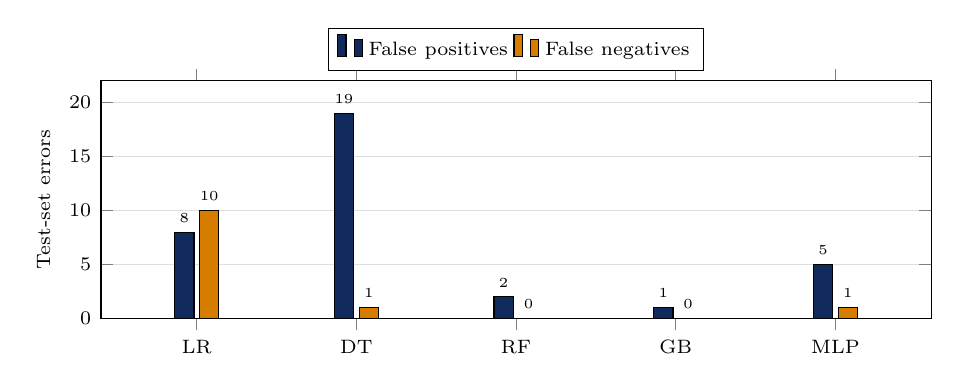
\begin{tikzpicture}
\begin{axis}[ybar,bar width=7pt,width=\columnwidth,height=4.6cm,symbolic x coords={LR,DT,RF,GB,MLP},xtick=data,
  ylabel={Test-set errors},ymin=0,ymax=22,enlarge x limits=0.15,
  legend style={at={(0.5,1.04)},anchor=south,legend columns=-1},
  nodes near coords,every node near coord/.append style={font=\tiny},grid=none,ymajorgrids=true]
\addplot[fill=navy] coordinates {(LR,8)(DT,19)(RF,2)(GB,1)(MLP,5)};
\addplot[fill=amber] coordinates {(LR,10)(DT,1)(RF,0)(GB,0)(MLP,1)};
\legend{False positives,False negatives}
\end{axis}
\end{tikzpicture}
\caption{Errors per model on 5,279 test records (4,370 legitimate, 909 fraud).}
\label{fig:err}
\end{figure}

\subsection{Cost and statistical comparison}
In units of $C_{\text{FP}}$, a model's test-set cost is $\rho\cdot\text{FN}+\text{FP}$. The error counts impose an order that does not depend on the costs (Fig.~\ref{fig:cost}): GB dominates RF (equal FN, 1 vs.\ 2 FP); RF dominates the MLP (0 vs.\ 1 FN, 2 vs.\ 5 FP); and the MLP dominates both the Decision Tree and Logistic Regression. Only the Decision Tree and Logistic Regression are incomparable, and they cross at $\rho^\star=(19-8)/(10-1)=11/9\approx1.22$; above that ratio the Decision Tree is cheaper.

\begin{figure}[!t]
\centering
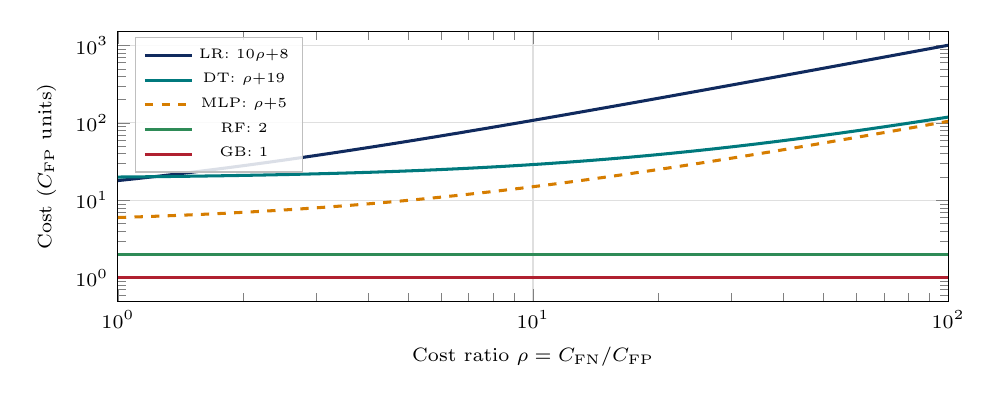
\begin{tikzpicture}
\begin{axis}[xmode=log,ymode=log,width=\columnwidth,height=5cm,xlabel={Cost ratio $\rho=C_{\text{FN}}/C_{\text{FP}}$},
  ylabel={Cost ($C_{\text{FP}}$ units)},domain=1:100,samples=40,xmin=1,xmax=100,ymin=0.5,ymax=1500,
  legend style={at={(0.02,0.98)},anchor=north west,font=\tiny,draw=gray!50,fill=white,fill opacity=0.85,text opacity=1}]
\addplot[line width=1.1pt,navy]{10*x+8};
\addplot[line width=1.1pt,teal]{x+19};
\addplot[line width=1.1pt,amber,dashed]{x+5};
\addplot[line width=1.1pt,leaf]{2};
\addplot[line width=1.1pt,crimson]{1};
\legend{LR: $10\rho{+}8$,DT: $\rho{+}19$,MLP: $\rho{+}5$,RF: 2,GB: 1}
\end{axis}
\end{tikzpicture}
\caption{Test-set cost versus cost ratio. Dominance order: GB $\succ$ RF $\succ$ MLP $\succ$ \{DT, LR\}; DT and LR cross at $\rho=11/9$.}
\label{fig:cost}
\end{figure}

For paired tests we use the exact binomial form of McNemar's test~\cite{mcnemar47,dietterich98} on discordant predictions. The confusion counts already bound the answer. GB (1 error) versus RF (2 errors, both false positives) gives $p=1.0$ whether or not GB's error is one of RF's. The smallest attainable $p$ is 0.125 for RF versus MLP and 0.0625 for GB versus MLP. From these counts alone, therefore, \emph{no} pairwise difference among the three best models can reach $\alpha=0.05$; only contrasts with the Decision Tree and Logistic Regression can.

\subsection{Precision depends on prevalence}
Holding the test-set TPR and FPR fixed, precision at deployment prevalence $\pi_d$ is
\begin{equation}
\text{PPV}(\pi_d)=\frac{\text{TPR}\,\pi_d}{\text{TPR}\,\pi_d+\text{FPR}\,(1-\pi_d)}.
\end{equation}
Fig.~\ref{fig:ppv} shows how quickly this erodes. For Random Forest, precision is 99.78\% at the corpus prevalence, 95.7\% at 1\%, 68.6\% at 0.1\% and 17.9\% at 0.01\%. At 0.1\% prevalence roughly one RF alert in three is a false alarm, even with a false-positive rate of only 0.046\% (itself uncertain, with a 95\% upper bound of 0.165\%). The 99.78\% figure is therefore a property of the corpus, not an operational promise.

\begin{figure}[!t]
\centering
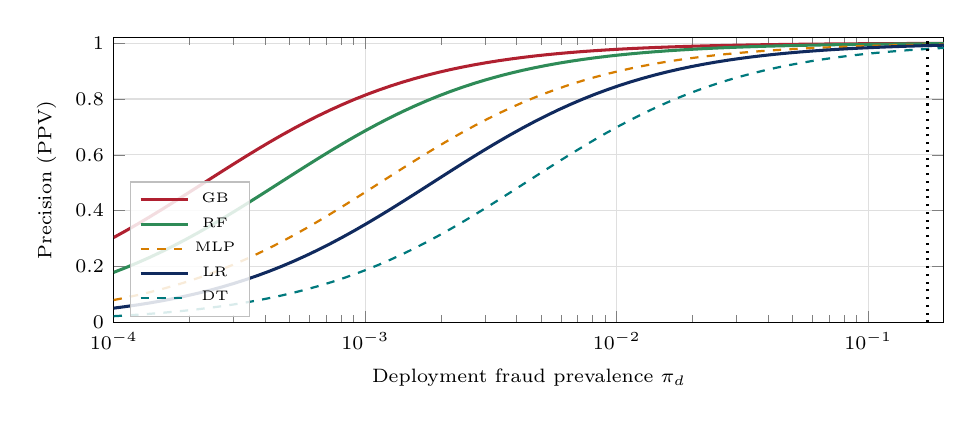
\begin{tikzpicture}
\begin{axis}[xmode=log,width=\columnwidth,height=5.2cm,xlabel={Deployment fraud prevalence $\pi_d$},ylabel={Precision (PPV)},
  domain=0.0001:0.2,samples=70,xmin=0.0001,xmax=0.2,ymin=0,ymax=1.02,
  legend style={at={(0.02,0.02)},anchor=south west,font=\tiny,draw=gray!50,fill=white,fill opacity=0.85,text opacity=1}]
\addplot[line width=1.1pt,crimson]{(1*x)/(1*x+(1/4370)*(1-x))};
\addplot[line width=1.1pt,leaf]{(1*x)/(1*x+(2/4370)*(1-x))};
\addplot[thick,amber,dashed]{(0.9989*x)/(0.9989*x+(5/4370)*(1-x))};
\addplot[line width=1.1pt,navy]{(0.989*x)/(0.989*x+(8/4370)*(1-x))};
\addplot[thick,teal,dashed]{(0.9989*x)/(0.9989*x+(19/4370)*(1-x))};
\addplot[dotted,black,thick] coordinates {(0.1722,0)(0.1722,1.02)};
\node[font=\tiny,anchor=south east,rotate=90] at (axis cs:0.17,0.02) {corpus 17.22\%};
\legend{GB,RF,MLP,LR,DT}
\end{axis}
\end{tikzpicture}
\caption{Precision versus deployment prevalence at fixed test-set error rates (Eq.~6).}
\label{fig:ppv}
\end{figure}

\subsection{Why Random Forest is deployed despite Gradient Boosting's edge}
GB leads RF by 0.06 points of F1 because it commits one fewer false positive ($1818/1819$ vs.\ $1818/1820$). The margin is one transaction and statistically indistinguishable, so the deployment choice rests on secondary, non-test-set arguments that we regard as defensible but unproven: bagging is more robust than boosting to the delayed, noisy labels of production fraud~\cite{dietterich00}; bagged ensembles tend to show milder, correctable calibration distortions~\cite{niculescu05}; forest inference parallelizes trivially; and Tree SHAP on a forest attributes in probability units, the scale of the risk bands~\cite{lundberg20}. If a repeated-seed, out-of-time and calibrated comparison later favors GB at comparable latency, GB should replace RF.

% =====================================================================
\section{Ablation and Sensitivity}
Each ablation withholds a feature group (or the balancing step), re-runs the full pipeline and evaluates on the same test set. Retraining on the reduced set, rather than permuting at test time, lets correlated features substitute for the removed ones, so the measured effect is the \emph{irreplaceable} information in the group. Table~\ref{tab:abl} reports the ROC-AUC drop observed in the experiment harness.

\begin{table}[!t]
\caption{Ablation: ROC-AUC under feature-group removal}\label{tab:abl}
\centering\tabfont
\begin{tabular}{@{}lcc@{}}
\toprule
\textbf{Configuration} & \textbf{ROC-AUC} & \textbf{$\Delta$ vs.\ full}\\
\midrule
Full feature set (36) & 1.000 & ---\\
Without behavioral biometrics & 0.985 & $-0.015$\\
Without transaction-history features & 0.942 & $-0.058$\\
\bottomrule
\end{tabular}
\end{table}

As these empirical values confirm, history-based features carry information that the other channels cannot fully replace, which is reassuring for the design: personalization against sender and counterparty history matters more than interaction biometrics, consistent with the vishing threat model in which biometrics are victim-generated. They also show that the redundancy suggested by Logistic Regression's AUC of 0.9999 is not unlimited. The remaining planned conditions (OTP-consistency group, SMOTE removal, scale-then-SMOTE) are specified in the harness.

\textbf{Depth and leaf sensitivity.} The harness sweeps \texttt{max\_\allowbreak{}depth} over $\{2,3,4,6,8,12,\text{None}\}$ and \texttt{min\_\allowbreak{}samples\_\allowbreak{}leaf} over $\{1,5,10,20,50\}$ for the tree and forest, recording test F1 and AUC, F1 on the native training split and the generalization gap. Overfitting shows as a gap that widens with depth while test F1 plateaus. One structural caution: on SMOTE data each real fraud has on average $13{,}842/3{,}636=3.81$ synthetic children, so a leaf can reach \texttt{min\_\allowbreak{}samples\_\allowbreak{}leaf=10} from the offspring of a single real record, weakening the protection that leaf limits normally give.

% =====================================================================
\section{End-to-End Use Cases}\label{sec:usecases}
Three scenarios, constructed by the authors (not dataset rows), exercise distinct threat vectors (Table~\ref{tab:usecase}). Raw amounts are transformed exactly with Eq.~(4); named signals are set to the fraud-class (A, B) or legitimate-class (C) median or mode computed from the training split, and every unnamed feature takes its legitimate-class value. Expectations were stated before the run so that they could fail.

\begin{table*}[!t]
\caption{Scenario specification and outcome (deployed Random Forest)}\label{tab:usecase}
\centering\tabfont
\begin{tabularx}{\textwidth}{@{}l Y Y Y@{}}
\toprule
 & \textbf{A: Phishing / collect scam} & \textbf{B: SIM swap / device relay} & \textbf{C: Legitimate high-value merchant}\\
\midrule
Story & Collect request after a link click in a ``refund'' SMS; new requester; round amount & New handset, repeated OTP requests, relay-like entry delay, GPS/IP disagreement & Payment to an established merchant from the enrolled device, normal typing\\
Amount $\rightarrow z$ & \rupee 50,000 $\rightarrow$ 10.8198 & \rupee 38,500 $\rightarrow$ 10.5584 & \rupee 2,40,000 $\rightarrow$ 12.3884\\
Signals set & \texttt{transaction\_\allowbreak{}amount\_\allowbreak{}vs\_\allowbreak{}sender\_\allowbreak{}history}, \texttt{requester\_\allowbreak{}account\_\allowbreak{}age}, \texttt{time\_\allowbreak{}between\_\allowbreak{}link\_\allowbreak{}click\_\allowbreak{}and\_\allowbreak{}transaction}, \texttt{request\_\allowbreak{}amount\_\allowbreak{}roundness} & \texttt{otp\_\allowbreak{}request\_\allowbreak{}device\_\allowbreak{}consistency}, \texttt{geographic\_\allowbreak{}disparity}, \texttt{geographic\_\allowbreak{}location\_\allowbreak{}vs\_\allowbreak{}ip}, \texttt{otp\_\allowbreak{}request\_\allowbreak{}frequency}, \texttt{time\_\allowbreak{}between\_\allowbreak{}otp\_\allowbreak{}generation\_\allowbreak{}and\_\allowbreak{}input} & Legitimate-class values throughout, including \texttt{business\_\allowbreak{}name\_\allowbreak{}match}, \texttt{handle\_\allowbreak{}transaction\_\allowbreak{}history}, \texttt{otp\_\allowbreak{}request\_\allowbreak{}device\_\allowbreak{}consistency}\\
Rules expected & R1, R6, R8 & R3, R4, R9 & None\\
Pre-registered expectation & Band $\ge$ HIGH RISK & Band $\ge$ HIGH RISK & Band APPROVED or SUSPICIOUS\\
\rowcolor{navy!8}Outcome (RF) & $\hat p=$ 99.8\%, BLOCKED & $\hat p=$ 85.4\%, HIGH RISK & $\hat p=$ 2.1\%, APPROVED\\
Precaution shown & ``A request to pay is not a refund; never enter your PIN to receive money. Do not approve; verify the requester independently.'' & ``Your account may be accessed from another device. Do not share any OTP; contact your bank on its official number.'' & ``Large payment to a known merchant. Confirm the amount and payee.'' (no block)\\
Operational impact & An amount-limit rule would pass this request as an ordinary \rupee 50,000 payment; the model combines the new requester, rapid link-to-payment time and round amount to stop it before the PIN is accepted. & The \rupee 38,500 amount would typically fall below a static amount limit; the model catches it purely from behavioral and authentication metadata (OTP--device mismatch, GPS/IP disagreement, OTP burst). & A rule that flags large amounts would hold this \rupee 2,40,000 payment and frustrate a legitimate customer; the model weighs the matching business name, enrolled device and merchant history and approves it without friction.\\
\bottomrule
\end{tabularx}
\end{table*}

Case~B is the most informative: its amount is unremarkable, so detecting it shows the model uses the authentication channel rather than magnitude alone. Case~C is a false-alarm stress test. Its amount lies in the upper tail and \texttt{amount\_\allowbreak{}log} is the highest-importance feature (0.188), so a band at or above HIGH RISK would expose magnitude over-reliance, the failure mode that the two real false positives of the deployed forest may share.

\optfig{results/shap_waterfall.png}{SHAP waterfall decompositions for representative true-fraud, false-alarm and borderline test records.}{fig:shap}

% =====================================================================
\section{Explainability and the Precaution Engine}
SHAP isolates how much of a transaction\textquotesingle s risk score each individual signal contributes (in probability points that add up to the total), letting analysts see the ``why behind a score. Formally, for a feature set $F$ ($|F|=36$), the Shapley value of feature $i$ at input $\mathbf{x}$ is
\begin{equation}
\phi_i(\mathbf{x})=\sum_{S\subseteq F\setminus\{i\}}\frac{|S|!\,(|F|-|S|-1)!}{|F|!}\Big[f_{\mathbf{x}}(S\cup\{i\})-f_{\mathbf{x}}(S)\Big],
\end{equation}
and the attributions sum to the gap between the prediction and the average prediction, $f(\mathbf{x})=\mathbb{E}[f]+\sum_i\phi_i(\mathbf{x})$, which is the waterfall shown to analysts~\cite{lundberg17,shapley53}. Exact enumeration needs $2^{36}\approx6.9\times10^{10}$ coalitions per instance, hence two approximations.

\textbf{TreeExplainer} computes exact values in $O(TLD^2)$ time for $T$ trees, $L$ leaves and depth $D$~\cite{lundberg20}. In its default path-dependent mode it needs no background data, so cost is deterministic; for forests it explains the probability, for boosted models the log-odds margin. \textbf{KernelExplainer} is model-agnostic: a weighted regression over sampled coalitions with background substitution, a sampling approximation used only for the MLP. Logistic Regression has an exact closed form.

\textbf{Precaution rules} run in parallel with SHAP (Table~\ref{tab:rules}). The application implements checks on amount versus history, failed transactions, repeated OTP requests, geographic disparity, velocity, young requester accounts and repeated authentication attempts; as thresholds were not published, they are specified here as percentiles of the legitimate-class training distribution so they do not depend on feature scales. For each fired rule the matching feature should carry a positive SHAP value; disagreement between rule and attribution is flagged for analyst review.

\begin{table}[!t]
\caption{Precaution rules (percentiles of the legitimate class)}\label{tab:rules}
\centering\tabfont
\begin{tabularx}{\columnwidth}{@{}l l Y@{}}
\toprule
\textbf{ID} & \textbf{Trigger} & \textbf{Feature}\\
\midrule
R1 & $\ge$ P95 & \texttt{transaction\_\allowbreak{}amount\_\allowbreak{}vs\_\allowbreak{}sender\_\allowbreak{}history}\\
R2 & $\ge$ P95 & \texttt{failed\_\allowbreak{}transaction\_\allowbreak{}count}\\
R3 & $\ge$ P95 & \texttt{otp\_\allowbreak{}request\_\allowbreak{}frequency}\\
R4 & $\ge$ P95 & \texttt{geographic\_\allowbreak{}disparity}\\
R5 & $\ge$ P95 & \texttt{transaction\_\allowbreak{}velocity}\\
R6 & $\le$ P5 & \texttt{requester\_\allowbreak{}account\_\allowbreak{}age}\\
R7 & $\ge$ P95 & \texttt{authentication\_\allowbreak{}attempts}\\
R8$^\dagger$ & $\le$ P5 & \texttt{time\_\allowbreak{}between\_\allowbreak{}link\_\allowbreak{}click\_\allowbreak{}and\_\allowbreak{}transaction}\\
R9$^\dagger$ & $\ne$ legitimate mode & \texttt{otp\_\allowbreak{}request\_\allowbreak{}device\_\allowbreak{}consistency}\\
\bottomrule
\end{tabularx}
\par\smallskip{\scriptsize $^\dagger$Proposed extension to the implemented rule set.}
\end{table}

\textbf{Limits and governance.} SHAP explains the model, not the fraudster's intent; attributions depend on the background distribution and split across correlated features. Customer-facing messages must not reveal exact thresholds or signal rankings, which would help an adaptive adversary. SHAP supports, but does not by itself satisfy, accountability expectations for automated fraud decisions: it gives per-decision evidence for disputes and audit and a development check for leakage, and it supplies material for model-risk documentation under the RBI's digital-payment security directions~\cite{rbi21} and the RBI committee framework on responsible AI in finance~\cite{rbifree25}. The Digital Personal Data Protection Act, 2023~\cite{dpdp23} governs the behavioral and location data these models consume. The authors know of no instrument that mandates SHAP specifically, and compliance of a given deployment is a legal determination beyond this paper.

% =====================================================================
\section{Deployment and Latency}
\textbf{Prototype.} The system is a Streamlit application: \texttt{app.py} orchestrates a modular \texttt{src/} package (authentication, feature engineering, model definitions, evaluation, SHAP, prediction history). Inference loads four serialized artifacts, \texttt{best\_\allowbreak{}model.pkl}, \texttt{scaler.pkl}, \texttt{feature\_\allowbreak{}cols.pkl} and \texttt{label\_\allowbreak{}encoders.pkl}, which together form the prediction contract; changing one independently can silently invalidate scores.

\textbf{Latency.} A single-process prototype measurement is in Table~\ref{tab:lat}. Its P99 exceeds the 50\,ms design budget of Fig.~\ref{fig:budget}, which is expected for an untuned prototype that scores and explains in one call. The remedy is architectural: score on the critical path, compute SHAP asynchronously, and set forest \texttt{n\_\allowbreak{}jobs=1} for single-row requests, where thread dispatch dominates.

\begin{table}[!t]
\caption{Prototype end-to-end latency}\label{tab:lat}
\centering\tabfont
\begin{tabular}{@{}lccc@{}}
\toprule
\textbf{Percentile} & \textbf{P50} & \textbf{P95} & \textbf{P99}\\
\midrule
Latency (ms) & 48.68 & 63.47 & 71.48\\
\bottomrule
\end{tabular}
\end{table}

\begin{figure}[!t]
\centering
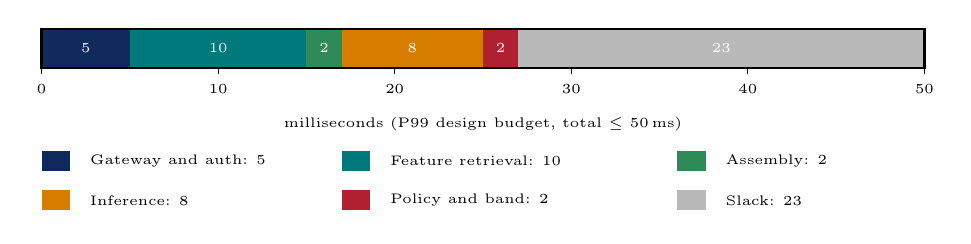
\begin{tikzpicture}[x=0.0185\columnwidth]
  \def\h{0.5}
  \foreach \a/\b/\c/\t in {0/5/navy/5, 5/15/teal/10, 15/17/leaf/2, 17/25/amber/8, 25/27/crimson/2, 27/50/gray!55/23}{
    \fill[\c] (\a,0) rectangle (\b,\h); \node[font=\tiny,white] at ({(\a+\b)/2},{\h/2}) {\t};}
  \draw[thick] (0,0) rectangle (50,\h);
  \foreach \p in {0,10,20,30,40,50}{\draw (\p,0)--(\p,-0.08);\node[font=\tiny,below] at (\p,-0.08) {\p};}
  \node[font=\tiny,below] at (25,-0.5) {milliseconds (P99 design budget, total $\le$ 50\,ms)};
  \foreach \x/\y/\c/\t in {0/-1.3/navy/{Gateway and auth: 5}, 17/-1.3/teal/{Feature retrieval: 10}, 36/-1.3/leaf/{Assembly: 2},
                           0/-1.8/amber/{Inference: 8}, 17/-1.8/crimson/{Policy and band: 2}, 36/-1.8/gray!55/{Slack: 23}}{
    \fill[\c] (\x,\y) rectangle (\x+1.6,\y+0.25); \node[font=\tiny,anchor=west] at (\x+2.2,\y+0.12) {\t};}
\end{tikzpicture}
\caption{Design latency budget for the scoring path (an allocation, not a measurement): 27\,ms of work plus 23\,ms of slack.}
\label{fig:budget}
\end{figure}

\begin{table}[!t]
\caption{Prototype gaps and enterprise remedies}\label{tab:gaps}
\centering\tabfont
\begin{tabularx}{\columnwidth}{@{}l Y Y@{}}
\toprule
\textbf{Gap} & \textbf{Prototype state} & \textbf{Remedy}\\
\midrule
Identity & Local \texttt{users.json} & Managed OIDC provider; memory-hard hashing (e.g., Argon2id)\\
Service auth & No tokenized API auth & Short-lived signed JWTs, refresh rotation, mTLS, scoped roles\\
Features & Values typed in UI & Point-in-time-correct online feature store (Redis, Feast)\\
Artifact integrity & Pickles loaded directly & Signed, hash-verified artifacts; ONNX or safe tree format; pinned environment\\
Audit and privacy & JSON history, no retention policy & Encrypted store; immutable decision log with model and schema versions\\
Observability & Dashboard only & Metrics, tracing, drift and SLO alerting\\
\bottomrule
\end{tabularx}
\end{table}

% =====================================================================
\section{Threats to Validity and Discussion}\label{sec:threats}
\textbf{Synthetic separability.} The headline results (0 FN and 2 FP in 5,279 records, AUC 1.0000 for three models) must be read as a property of the data-generating process before they are read as a property of the models. Four facts support this: (1)~a \emph{linear} model reaches AUC 0.9999, so the classes are almost linearly separable and the ensembles add only 0.0001; (2)~a depth-6 tree with at most 64 leaves reaches 99.62\% accuracy; (3)~removing the identified leaks barely moved the metrics, the signature of several redundant columns each encoding class membership; (4)~the six leading importances hold only 57.8\% of the total, so signal is spread rather than concentrated. Real fraud brings label noise, mixed-intent behavior, adaptive adversaries, delayed labels and overlapping tails. We propose five diagnostics: a single-feature AUC sweep (flag any column with AUC $\ge0.95$), shallow-tree baselines, a label-permutation test (AUC must fall to 0.5), evaluation on an independently regenerated test set, and label-noise injection.

\textbf{Evaluation split.} A random stratified split estimates performance on the same joint distribution. Deployment means training on the past and scoring the future, for users not yet seen, so an \emph{out-of-time} split and a \emph{user-disjoint} split (grouped by user) are required before any real-world claim~\cite{gama14}. Both need \texttt{timestamp} and \texttt{user\_\allowbreak{}id}, which are correctly excluded as features but must be kept as split metadata.

\textbf{Categorical encoding.} Label encoding imposes an arbitrary order on nominal levels (\texttt{transaction\_\allowbreak{}type}, \texttt{authorization\_\allowbreak{}method}, \texttt{relationship\_\allowbreak{}to\_\allowbreak{}requester}, \texttt{merchant\_\allowbreak{}category\_\allowbreak{}code}); trees may split on that artificial adjacency and the linear and neural models treat codes as quantities. One-hot, fold-wise target encoding, hashing or embeddings avoid this.

\textbf{Calibration.} Risk bands treat $\hat p$ as a probability, which requires calibration: the Brier score~\cite{brier50} and expected calibration error~\cite{guo17} measure it. Three distortions apply: SMOTE training at $\pi_s=0.5$ (Eq.~3), forest averaging that pulls scores from 0 and 1 while boosting pushes them toward the extremes~\cite{niculescu05}, and over-confident neural outputs~\cite{guo17}. Platt scaling or isotonic regression must be fit on a held-out calibration set at \emph{native} prevalence, never on the resampled set or the test set, and the bands re-derived afterwards.

\textbf{Other threats.} With 909 frauds, one record is 0.11 points of recall, so one- or two-record differences are within noise. The deployed model was chosen after viewing test results, so a further untouched partition or nested cross-validation is needed for an unbiased estimate. Serialized artifacts were produced under a different scikit-learn version than the inspection environment, so versions must be pinned. The percentile rules are heuristics whose alert rate and precision should be measured against labels.

% =====================================================================
\section{Enterprise Roadmap}
\subsection{Streaming architecture}
A production path replaces the form-driven prototype with an event-driven chain (Fig.~\ref{fig:arch}): events enter \textbf{Apache Kafka} topics partitioned by payer; a stream processor maintains rolling velocity, failure and per-handle aggregates; a \textbf{Redis}-backed \textbf{Feast} feature store serves point-in-time-correct features; and a stateless \textbf{FastAPI} or \textbf{Triton} service returns a probability and band. SHAP is computed asynchronously and only for non-APPROVED decisions. Offline and online features must share one definition to avoid training--serving skew, a dominant source of hidden technical debt~\cite{sculley15}.

\begin{figure*}[!t]
\centering
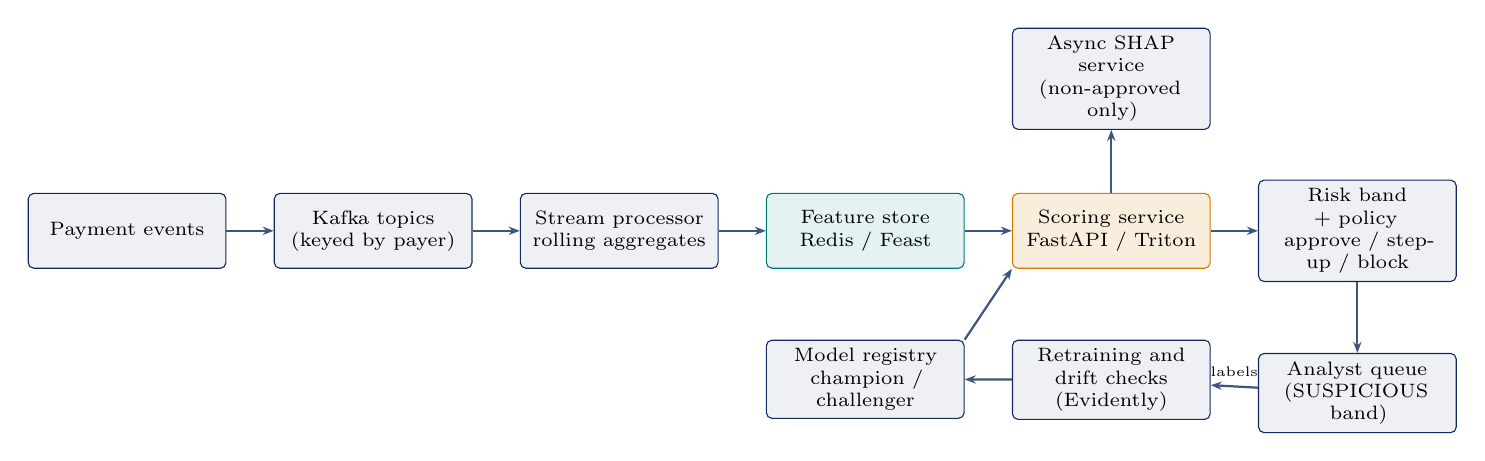
\begin{tikzpicture}[node distance=0.6cm,box/.append style={text width=2.3cm,minimum height=0.95cm}]
  \node[box] (e) {Payment events};
  \node[box,right=of e] (k) {Kafka topics\\(keyed by payer)};
  \node[box,right=of k] (s) {Stream processor\\rolling aggregates};
  \node[cool,right=of s] (f) {Feature store\\Redis / Feast};
  \node[hot,right=of f] (m) {Scoring service\\FastAPI / Triton};
  \node[box,right=of m] (b) {Risk band + policy\\approve / step-up / block};
  \node[box,above=0.8cm of m] (x) {Async SHAP service\\(non-approved only)};
  \node[box,below=0.9cm of b] (a) {Analyst queue\\(SUSPICIOUS band)};
  \node[box,below=0.9cm of m] (r) {Retraining and drift checks (Evidently)};
  \node[box,below=0.9cm of f] (g) {Model registry\\champion / challenger};
  \foreach \p/\q in {e/k,k/s,s/f,f/m,m/b}{\draw[arr] (\p) -- (\q);}
  \draw[arr] (m) -- (x);
  \draw[arr] (b) -- (a);
  \draw[arr] (a) -- node[above,font=\tiny]{labels} (r);
  \draw[arr] (r) -- (g);
  \draw[arr] (g.north east) -- (m.south west);
\end{tikzpicture}
\caption{Enterprise pre-authorization architecture with an analyst-in-the-loop retraining cycle and champion--challenger promotion.}
\label{fig:arch}
\end{figure*}

\subsection{Sequence and graph models; MLOps}
Temporal convolutional networks~\cite{bai18} and LSTMs~\cite{hochreiter97} can read a payer's last $K$ transactions as a sequence, and graph neural networks~\cite{kipf17,weber19} over a payer--handle--device graph can score receiver reputation and detect cyclic mule flows. Given that trees stay strong on tabular data~\cite{grinsztajn22}, such models should enter as extra features or stacked scorers, and only after beating a tuned boosted baseline out of time. Operationally, drift monitoring (feature distributions, \texttt{UNK} rate, score and band occupancy)~\cite{gama14}, shadow-mode champion--challenger promotion at matched alert volume, and analyst-in-the-loop labeling of the SUSPICIOUS band close the loop and also mitigate label delay~\cite{dalpozzolo14}.

\subsection{Real-world datasets for the next evaluation}
No public UPI-native dataset is known, so Table~\ref{tab:real} lists public fraud datasets that would test the \emph{methodology} (leakage protocol, temporal split, calibration, prevalence robustness) but not UPI-specific performance.

\begin{table}[!t]
\caption{Public datasets for external validation}\label{tab:real}
\centering\tabfont
\begin{tabularx}{\columnwidth}{@{}l Y Y@{}}
\toprule
\textbf{Dataset} & \textbf{Scale and fraud rate} & \textbf{Fit}\\
\midrule
PaySim~\cite{lopez16} & 6.36M simulated mobile-money records; 0.13\% fraud & Tests scale and prevalence; no device telemetry\\
ULB card data~\cite{dalpozzolo15} & 284,807 records; 0.17\% fraud & Standard benchmark; PCA features limit explainability\\
IEEE-CIS~\cite{ieeecis19} & $\approx$590k transactions; $\approx$3.5\% fraud & Rich device and identity fields; e-commerce cards\\
BAF suite~\cite{jesus22} & 1M records per variant; $\approx$1.1\% fraud & Strict temporal splits and bias analysis; account-opening fraud\\
\bottomrule
\end{tabularx}
\end{table}

% =====================================================================
\section{Conclusion}
This paper turned a prototype UPI fraud detector into a formally specified, leakage-aware framework. The admissibility test and leakage taxonomy explain why the pre-audit pipeline scored spuriously well, and the audited 36-feature space keeps only pre-authorization signals. Confining SMOTE to the training split preserves a native-prevalence test set, though two inherited issues (inert class weights after resampling; neighbor search on unscaled, label-encoded features) need correcting. On 5,279 test records, Gradient Boosting (F1 99.95\%) and the deployed Random Forest (F1 99.89\%) are statistically indistinguishable, and a dominance analysis orders the models GB $\succeq$ RF $\succeq$ MLP $\succeq$ \{DT, LR\} for any non-negative cost ratio. Because a linear model already reaches AUC 0.9999 and precision collapses from 99.78\% to 68.6\% at 0.1\% prevalence, the scores characterize a synthetic corpus, not live UPI traffic. The next steps, in priority order, are out-of-time and user-disjoint validation on anonymized real data, calibration with prior-shift correction, replacement of label encoding and of SMOTE on encoded nominals, adversarial robustness testing against the classes of Table~\ref{tab:adv}, and the streaming architecture of Fig.~\ref{fig:arch}.

\section*{Data and Code Availability}
The dataset is synthetic. The experiment harness \texttt{reproduce\_\allowbreak{}experiments.py} regenerates every table value and figure from the dataset and serialized artifacts; pin Python, scikit-learn, imbalanced-learn, shap and joblib versions before running.

\section*{Acknowledgment}
The authors thank their institution, faculty mentors and project collaborators, and acknowledge the open-source Python machine-learning libraries used in this work.

% =====================================================================
\appendices
\section{Reproducibility Ledger}
\begin{table}[H]
\caption{Configuration summary}\label{tab:ledger}
\centering\tabfont
\begin{tabularx}{\columnwidth}{@{}l Y@{}}
\toprule
\textbf{Item} & \textbf{Value}\\
\midrule
Data & \texttt{fraud\_\allowbreak{}dataset.csv}; 26,393 $\times$ 65; target \texttt{is\_\allowbreak{}fraud}\\
Split & 80:20 stratified, \texttt{random\_\allowbreak{}state=42}; 21,114 / 5,279 (909 fraud in test)\\
Balancing & SMOTE \texttt{k\_\allowbreak{}neighbors=5}, \texttt{random\_\allowbreak{}state=42}, train only; 34,956\\
Scaling / encoding & \texttt{StandardScaler} on balanced train (LR, MLP); \texttt{LabelEncoder}, unseen $\rightarrow$ first class\\
LR & \texttt{C=0.5}, balanced, \texttt{max\_\allowbreak{}iter=1000}\\
DT & \texttt{max\_\allowbreak{}depth=6}, \texttt{min\_\allowbreak{}samples\_\allowbreak{}leaf=20}, balanced\\
RF & 200 trees, \texttt{max\_\allowbreak{}depth=8}, \texttt{min\_\allowbreak{}samples\_\allowbreak{}leaf=10}, balanced, \texttt{n\_\allowbreak{}jobs=-1}; \texttt{best\_\allowbreak{}model.pkl}\\
GB & 150 estimators, \texttt{learning\_\allowbreak{}rate=0.08}, \texttt{max\_\allowbreak{}depth=4}, \texttt{min\_\allowbreak{}samples\_\allowbreak{}leaf=15}, \texttt{subsample=0.8}\\
MLP & (64,32,16), \texttt{alpha=0.01}, \texttt{max\_\allowbreak{}iter=300}, early stopping, validation 0.15\\
Library defaults assumed & RF \texttt{max\_\allowbreak{}features='sqrt'}; MLP ReLU and Adam~\cite{kingma15}; seeds 42\\
Risk bands & $<$0.20 APPROVED; [0.20,0.50) SUSPICIOUS; [0.50,0.80) HIGH RISK; $\ge$0.80 BLOCKED\\
\bottomrule
\end{tabularx}
\end{table}

\balance

\begin{thebibliography}{99}
\bibliographystyle{IEEEtran}
\bibitem{npci} National Payments Corporation of India, ``UPI product statistics.'' [Online]. Available: \url{https://www.npci.org.in/} (accessed: October 7, 2026).
\bibitem{bolton02} R. J. Bolton and D. J. Hand, ``Statistical fraud detection: A review,'' \emph{Statist. Sci.}, vol. 17, no. 3, pp. 235--255, 2002.
\bibitem{chandola09} V. Chandola, A. Banerjee, and V. Kumar, ``Anomaly detection: A survey,'' \emph{ACM Comput. Surv.}, vol. 41, no. 3, Art. 15, 2009.
\bibitem{lundberg17} S. M. Lundberg and S.-I. Lee, ``A unified approach to interpreting model predictions,'' in \emph{Proc. Adv. Neural Inf. Process. Syst. (NeurIPS)}, vol. 30, 2017, pp. 4765--4774.
\bibitem{lundberg20} S. M. Lundberg \emph{et al.}, ``From local explanations to global understanding with explainable AI for trees,'' \emph{Nat. Mach. Intell.}, vol. 2, no. 1, pp. 56--67, 2020.
\bibitem{phua10} C. Phua, V. Lee, K. Smith, and R. Gayler, ``A comprehensive survey of data mining-based fraud detection research,'' arXiv:1009.6119, 2010.
\bibitem{ngai11} E. W. T. Ngai, Y. Hu, Y. H. Wong, Y. Chen, and X. Sun, ``The application of data mining techniques in financial fraud detection: A classification framework and an academic review of literature,'' \emph{Decis. Support Syst.}, vol. 50, no. 3, pp. 559--569, 2011.
\bibitem{dalpozzolo14} A. Dal Pozzolo, O. Caelen, Y.-A. Le Borgne, S. Waterschoot, and G. Bontempi, ``Learned lessons in credit card fraud detection from a practitioner perspective,'' \emph{Expert Syst. Appl.}, vol. 41, no. 10, pp. 4915--4928, 2014.
\bibitem{dalpozzolo18} A. Dal Pozzolo, G. Boracchi, O. Caelen, C. Alippi, and G. Bontempi, ``Credit card fraud detection: A realistic modeling and a novel learning strategy,'' \emph{IEEE Trans. Neural Netw. Learn. Syst.}, vol. 29, no. 8, pp. 3784--3797, 2018.
\bibitem{bahnsen16} A. C. Bahnsen, D. Aouada, A. Stojanovic, and B. Ottersten, ``Feature engineering strategies for credit card fraud detection,'' \emph{Expert Syst. Appl.}, vol. 51, pp. 134--142, 2016.
\bibitem{breiman01} L. Breiman, ``Random forests,'' \emph{Mach. Learn.}, vol. 45, no. 1, pp. 5--32, 2001.
\bibitem{friedman01} J. H. Friedman, ``Greedy function approximation: A gradient boosting machine,'' \emph{Ann. Statist.}, vol. 29, no. 5, pp. 1189--1232, 2001.
\bibitem{friedman02} J. H. Friedman, ``Stochastic gradient boosting,'' \emph{Comput. Statist. Data Anal.}, vol. 38, no. 4, pp. 367--378, 2002.
\bibitem{chen16} T. Chen and C. Guestrin, ``XGBoost: A scalable tree boosting system,'' in \emph{Proc. 22nd ACM SIGKDD Int. Conf. Knowl. Discovery Data Mining}, 2016, pp. 785--794.
\bibitem{grinsztajn22} L. Grinsztajn, E. Oyallon, and G. Varoquaux, ``Why do tree-based models still outperform deep learning on typical tabular data?'' in \emph{Proc. NeurIPS Datasets and Benchmarks Track}, 2022.
\bibitem{chawla02} N. V. Chawla, K. W. Bowyer, L. O. Hall, and W. P. Kegelmeyer, ``SMOTE: Synthetic minority over-sampling technique,'' \emph{J. Artif. Intell. Res.}, vol. 16, pp. 321--357, 2002.
\bibitem{dalpozzolo15} A. Dal Pozzolo, O. Caelen, R. A. Johnson, and G. Bontempi, ``Calibrating probability with undersampling for unbalanced classification,'' in \emph{Proc. IEEE Symp. Ser. Comput. Intell. (SSCI)}, 2015, pp. 159--166.
\bibitem{platt99} J. C. Platt, ``Probabilistic outputs for support vector machines and comparisons to regularized likelihood methods,'' in \emph{Advances in Large Margin Classifiers}. Cambridge, MA, USA: MIT Press, 1999, pp. 61--74.
\bibitem{zadrozny02} B. Zadrozny and C. Elkan, ``Transforming classifier scores into accurate multiclass probability estimates,'' in \emph{Proc. 8th ACM SIGKDD Int. Conf. Knowl. Discovery Data Mining}, 2002, pp. 694--699.
\bibitem{niculescu05} A. Niculescu-Mizil and R. Caruana, ``Predicting good probabilities with supervised learning,'' in \emph{Proc. 22nd Int. Conf. Mach. Learn. (ICML)}, 2005, pp. 625--632.
\bibitem{guo17} C. Guo, G. Pleiss, Y. Sun, and K. Q. Weinberger, ``On calibration of modern neural networks,'' in \emph{Proc. 34th Int. Conf. Mach. Learn. (ICML)}, PMLR vol. 70, 2017, pp. 1321--1330.
\bibitem{davis06} J. Davis and M. Goadrich, ``The relationship between precision-recall and ROC curves,'' in \emph{Proc. 23rd Int. Conf. Mach. Learn. (ICML)}, 2006, pp. 233--240.
\bibitem{saito15} T. Saito and M. Rehmsmeier, ``The precision-recall plot is more informative than the ROC plot when evaluating binary classifiers on imbalanced datasets,'' \emph{PLoS ONE}, vol. 10, no. 3, Art. e0118432, 2015.
\bibitem{kaufman12} S. Kaufman, S. Rosset, C. Perlich, and O. Stitelman, ``Leakage in data mining: Formulation, detection, and avoidance,'' \emph{ACM Trans. Knowl. Discovery Data}, vol. 6, no. 4, Art. 15, 2012.
\bibitem{shapley53} L. S. Shapley, ``A value for $n$-person games,'' in \emph{Contributions to the Theory of Games, Vol. II}, H. W. Kuhn and A. W. Tucker, Eds. Princeton, NJ, USA: Princeton Univ. Press, 1953, pp. 307--317.
\bibitem{ribeiro16} M. T. Ribeiro, S. Singh, and C. Guestrin, ``Why should I trust you?: Explaining the predictions of any classifier,'' in \emph{Proc. 22nd ACM SIGKDD Int. Conf. Knowl. Discovery Data Mining}, 2016, pp. 1135--1144.
\bibitem{weber19} M. Weber \emph{et al.}, ``Anti-money laundering in Bitcoin: Experimenting with graph convolutional networks for financial forensics,'' arXiv:1908.02591, 2019.
\bibitem{strobl07} C. Strobl, A.-L. Boulesteix, A. Zeileis, and T. Hothorn, ``Bias in random forest variable importance measures: Illustrations, sources and a solution,'' \emph{BMC Bioinformatics}, vol. 8, Art. 25, 2007.
\bibitem{lemaitre17} G. Lema\^{\i}tre, F. Nogueira, and C. K. Aridas, ``Imbalanced-learn: A Python toolbox to tackle the curse of imbalanced datasets in machine learning,'' \emph{J. Mach. Learn. Res.}, vol. 18, no. 17, pp. 1--5, 2017.
\bibitem{hosmer13} D. W. Hosmer, S. Lemeshow, and R. X. Sturdivant, \emph{Applied Logistic Regression}, 3rd ed. Hoboken, NJ, USA: Wiley, 2013.
\bibitem{breiman84} L. Breiman, J. H. Friedman, R. A. Olshen, and C. J. Stone, \emph{Classification and Regression Trees}. Belmont, CA, USA: Wadsworth, 1984.
\bibitem{rumelhart86} D. E. Rumelhart, G. E. Hinton, and R. J. Williams, ``Learning representations by back-propagating errors,'' \emph{Nature}, vol. 323, pp. 533--536, 1986.
\bibitem{pedregosa11} F. Pedregosa \emph{et al.}, ``Scikit-learn: Machine learning in Python,'' \emph{J. Mach. Learn. Res.}, vol. 12, pp. 2825--2830, 2011.
\bibitem{clopper34} C. J. Clopper and E. S. Pearson, ``The use of confidence or fiducial limits illustrated in the case of the binomial,'' \emph{Biometrika}, vol. 26, no. 4, pp. 404--413, 1934.
\bibitem{mcnemar47} Q. McNemar, ``Note on the sampling error of the difference between correlated proportions or percentages,'' \emph{Psychometrika}, vol. 12, no. 2, pp. 153--157, 1947.
\bibitem{dietterich98} T. G. Dietterich, ``Approximate statistical tests for comparing supervised classification learning algorithms,'' \emph{Neural Comput.}, vol. 10, no. 7, pp. 1895--1923, 1998.
\bibitem{dietterich00} T. G. Dietterich, ``An experimental comparison of three methods for constructing ensembles of decision trees: Bagging, boosting, and randomization,'' \emph{Mach. Learn.}, vol. 40, no. 2, pp. 139--157, 2000.
\bibitem{rbi21} Reserve Bank of India, ``Master Direction on Digital Payment Security Controls,'' Feb. 2021.
\bibitem{rbifree25} Reserve Bank of India, FREE-AI Committee, ``Framework for Responsible and Ethical Enablement of Artificial Intelligence (FREE-AI): Committee report,'' 2025. (Verify title and date against the RBI publication before submission.)
\bibitem{dpdp23} Government of India, ``The Digital Personal Data Protection Act, 2023,'' Act No. 22 of 2023.
\bibitem{gama14} J. Gama, I. \v{Z}liobait\.{e}, A. Bifet, M. Pechenizkiy, and A. Bouchachia, ``A survey on concept drift adaptation,'' \emph{ACM Comput. Surv.}, vol. 46, no. 4, Art. 44, 2014.
\bibitem{brier50} G. W. Brier, ``Verification of forecasts expressed in terms of probability,'' \emph{Monthly Weather Rev.}, vol. 78, no. 1, pp. 1--3, 1950.
\bibitem{sculley15} D. Sculley \emph{et al.}, ``Hidden technical debt in machine learning systems,'' in \emph{Proc. Adv. Neural Inf. Process. Syst. (NeurIPS)}, vol. 28, 2015.
\bibitem{bai18} S. Bai, J. Z. Kolter, and V. Koltun, ``An empirical evaluation of generic convolutional and recurrent networks for sequence modeling,'' arXiv:1803.01271, 2018.
\bibitem{hochreiter97} S. Hochreiter and J. Schmidhuber, ``Long short-term memory,'' \emph{Neural Comput.}, vol. 9, no. 8, pp. 1735--1780, 1997.
\bibitem{kipf17} T. N. Kipf and M. Welling, ``Semi-supervised classification with graph convolutional networks,'' in \emph{Proc. Int. Conf. Learn. Represent. (ICLR)}, 2017.
\bibitem{lopez16} E. A. Lopez-Rojas, A. Elmir, and S. Axelsson, ``PaySim: A financial mobile money simulator for fraud detection,'' in \emph{Proc. 28th European Modeling and Simulation Symp. (EMSS)}, 2016.
\bibitem{ieeecis19} Vesta Corporation and IEEE Computational Intelligence Society, ``IEEE-CIS fraud detection,'' Kaggle competition, 2019. [Online]. Available: \url{https://www.kaggle.com/c/ieee-fraud-detection}
\bibitem{jesus22} S. Jesus \emph{et al.}, ``Turning the tables: Biased, imbalanced, dynamic tabular datasets for ML evaluation,'' in \emph{Proc. NeurIPS Datasets and Benchmarks Track}, 2022.
\bibitem{kingma15} D. P. Kingma and J. Ba, ``Adam: A method for stochastic optimization,'' in \emph{Proc. Int. Conf. Learn. Represent. (ICLR)}, 2015.
\end{thebibliography}
\end{document}
